\documentclass[11pt]{article}
\usepackage[margin=0.75in]{geometry}
\usepackage{graphicx}
\usepackage{parskip}
\usepackage{hyperref}
\usepackage{breakurl}
\hypersetup{
    colorlinks=true,
    linkcolor=blue,
    filecolor=magenta,      
    urlcolor=cyan,
    pdftitle={USGS \LaTeX Installation Instructions},
    pdfpagemode=FullScreen,
    }
\parskip=1.00\baselineskip \advance\parskip by 0pt plus 2pt
\newcommand{\MacOSX}{\mbox{MacOSX}}
\usepackage[OT1]{fontenc}

\graphicspath{{./figures/}}


\begin{document}
\renewcommand\sfdefault{fun}


\begin{centering}
\noindent \textsf{\bfseries \Large Installation of Univers Condensed Font Library \\ and USGS Style Files for} \TeX/\LaTeX \\
\normalsize  \textsf{\bfseries \today \\}
\end{centering}

\addvspace{\baselineskip}

\section*{\textsf{Installation Instructions}}

\begin{enumerate}

	\item The installation instructions assume that you have already installed the \TeX~Live distribution available from \url{https://www.tug.org/texlive/} for \texttt{Linux} and \texttt{Windows} or the Mac\TeX~distribution available from \url{https://www.tug.org/mactex/} for \texttt{MacOS}. A minimal \TeX~Live distribution, sufficient for the Univers Condensed font library and USGS style files, can also be installed for many \texttt{Linux} distros using
	
	\begin{verbatim}
	  sudo apt install texlive-latex-extra texlive-science
	\end{verbatim}
	 
	These installation installation instructions may work for other \TeX~distributions but this has not been tested.
	
	\item Clone the \href{https://github.com/MODFLOW-USGS/usgslatex}{\texttt{usgslatex}} repository to a location of your choice on your computer. On \texttt{Windows}, the \texttt{usgslatex} repository should be cloned to your \texttt{C:} drive for the installation file to work correctly.
	
	\item Install the Univers Condensed font library and USGS style files
	
	\begin{enumerate}
	
		\item To install the Univers Condensed font library and USGS style files on \texttt{MacOS} or \texttt{Linux} open a terminal in the \texttt{usgsLaTeX} subdirectory in your local clone of the \texttt{usgslatex} repository and type
		
		\begin{verbatim}
		  sudo ./install.sh
		\end{verbatim}
		
		\texttt{sudo} is required to modified system files (for example, \texttt{/usr/local/texlive/2021/texmf-var/fonts/}) for a specific \TeX~Live distribution.
		
		
		\item To install the Univers Condensed font library and USGS style files on \texttt{Windows}, run \texttt{install.bat} in the \texttt{usgsLaTeX} subdirectory in your local clone of the \texttt{usgslatex} repository as an Adminstrator by right-clicking on the file and selecting ``Run as administration'', as shown in figure~\ref{fig:windows-install}.
		
		
		\begin{figure}[!htbp]
		\begin{center}
			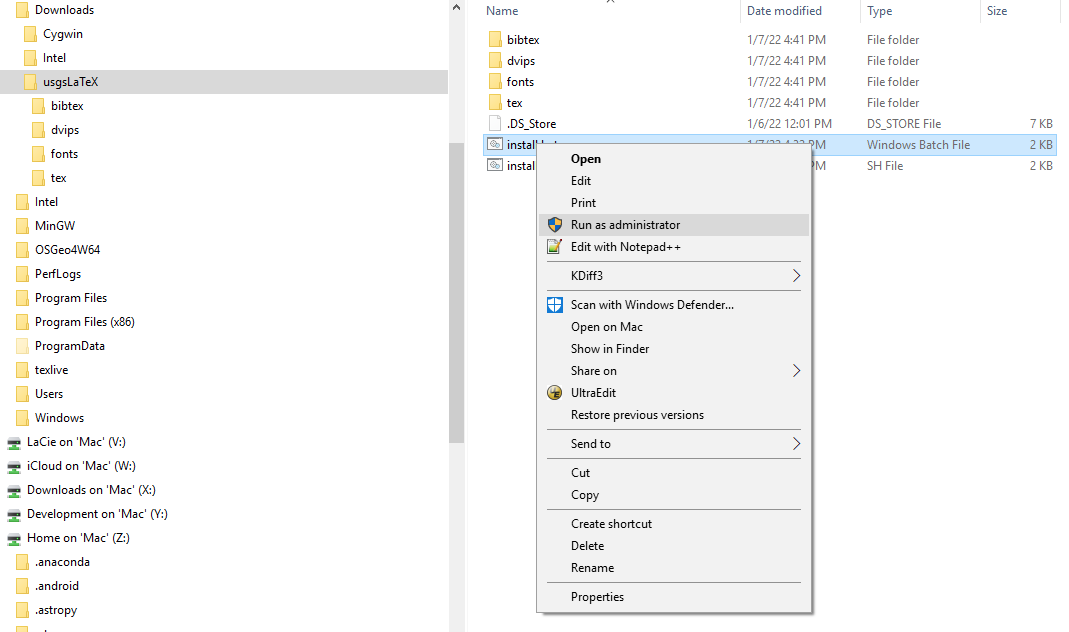
\includegraphics[scale=0.25]{windows_admin_install}
		\caption{Installation of the Univers Condensed Font Library and USGS Style Files for \TeX/\LaTeX~on \texttt{Windows} using the \texttt{install.bat} batch file.}
		\label{fig:windows-install}
		\end{center}
		\end{figure}
			
		Similar to installing the Univers Condensed font library and USGS style files on \texttt{MacOS} and \texttt{Linux}, \texttt{install.bat} is run as an Administrator so that system files can be modified.
	
	\end{enumerate}
	
	\item If the USGS style files have been correctly installed you should see something like the following on the last three lines of the output from \texttt{install.sh} and \texttt{install.bat}.
	
	\begin{enumerate}
	
		\item On \texttt{MacOS} and \texttt{Linux} you should see something like
		
		\begin{verbatim}
		  
		  Evaluate if USGS style files are available
		  Location of USGS LaTeX style files:  
		  /Users/jdhughes/Library/texmf/tex/latex/usgs/usgsreporta.sty
		\end{verbatim}
		
		\item On \texttt{Windows} you should see something like
		
		\begin{verbatim}
		
		  Evaluate if USGS style files are available
		  Location of USGS LaTeX style files:  
		  c:/texlive/texmf-local/tex/latex/usgs/usgsreporta.sty
		\end{verbatim}
	
	\end{enumerate}
	
	\item Test the Installation of the Univers Condensed font library installation can be tested using the \texttt{testunivers.tex} \TeX file in the \texttt{test} subdirectory. The file \texttt{testunivers.tex} is self contained in its definition of the Univers family, and does not use a separate package file. Try running \texttt{testunivers.tex} file through \LaTeX\ by typing \texttt{pdflatex testunivers.tex} in a terminal open in the \texttt{test} subdirectory (or your preferred method of compiling  \TeX~files). Inspect the \texttt{testunivers.pdf} file. Compare the content of the generated \textsf{pdf} file to \texttt{testuniversPROOF.pdf}. If these two \textsf{pdf} files appear different the Univers font family was not installed correctly. 
	
	Refer to William Asquith's original font installation document (\texttt{README\_FontLibraryInstallation.pdf}) in the \texttt{doc} subdirectory  for more details on installing the Univers Condensed Font Library if it was not successfully installed by \texttt{install.sh} and \texttt{install.bat}.
	
	\item The file \texttt{USGSLaTeXReport.tex} is a more complicated test of successful installation of the USGS Style files. Try running \texttt{USGSLaTeXReport.tex} file through \LaTeX\ using your preferred method of compiling  \TeX~files. Inspect the \texttt{USGSLaTeXReport.pdf} file. Compare the content of the generated \textsf{pdf} file to \texttt{USGSLaTeXReportPROOF.pdf}. If these two \textsf{pdf} files appear different then there is a problem with your installation. Confirm that the USGS style files (in the \texttt{\$TEXROOT/tex/latex/usgs}) subdirectory. \texttt{\$TEXROOT} can be determined on \texttt{MacOS} and \texttt{linux} by typing the following in a terminal:
	
	\begin{verbatim}
		kpsewhich -var-value TEXMFHOME
	\end{verbatim}
	
	\texttt{\$TEXROOT} can be determined on \texttt{Windows} by typing the following in a terminal:

	\begin{verbatim}
		kpsewhich -var-value TEXMFLOCAL
	\end{verbatim}


\end{enumerate}

\section*{\textsf{Using the USGS Style Files}}
A simple example for using the \LaTeX~USGS style files is included in \texttt{doc/README\_USGSstyFILES.pdf}. Individual style files in the package are also listed and described in \texttt{doc/README\_USGSstyFILES.pdf}.

\section*{\textsf{Updating an existing installation}}
On \texttt{MacOS}, an existing installation can be updated by:

\begin{enumerate}
	\item Moving the existing installation (for example, \texttt{/usr/local/texlive/2014/}) to the trash.
	\item Move all existing \LaTeX\ software (for example, \texttt{TeXShop}) to the trash.
	\item Empty trash
	\item Install the new distribution
	\item Open the \TeX Live Utility and
	\begin{enumerate}
		\item Update the \TeX Live Utility and allow any infrastructure updates
		\item Install the \texttt{graphics-def} package if it is not installed
		\item Update all installed packages
	\end{enumerate}
	\item Open a terminal in \texttt{\$TEXROOT/dvips/funivers/} directory and type the following with \texttt{sudo} privileges to allow the new version of \LaTeX\ to access the Univers Condensed Font library
	\begin{enumerate}
		\item \texttt{texhash}
		\item \texttt{updmap -sys --enable Map=funivers.map}
		\item \texttt{updmap-sys}
	\end{enumerate}
\end{enumerate}


\section*{\textsf{Acknowledgements}}

The USGS Style files and instructions for installing the Univers Condensed Font library were originally developed by William H. Asquith in the Texas Water Science Center. The USGS style files have been subsequently modified by Michael N. Fienen (Wisconsin Water Science Center), Christian D. Langevin (Water Resources Mission Area), and Joseph D. Hughes (Water Resources Mission Area) to add additional functionality and maintain consistency with SPN guidelines. 

\end{document}
